\section{Enhancements to CODA in version 4.0.0}
\label{sec:component_diagrams-enhancements}
This section describes enhancements that were introduced into the CODA component diagram modelling tool as a result of experience. These enhancements were introduced in version 4.0.0 of CODA.

\subsection{Multiple Self Wake queues}
In previous CODA versions, a component owned one implicit queue of wake events. This meant that it was not possible to distinguish between wake events sent for different (domain level) purposes. A component may now own several different wake queues, which are added by the user to represent different self-wake semantics (Figure \ref{fig:Wake QueuesAreAddedToAComponentUsingThePalette}). SelfWake operations must specify which of the component's wake queues they wake on (Figure \ref{fig:SelfWakeOperationsMustSpecifyWhichOfTheComponentsWakeQueuesTheyWakeOn}), and Operations that set a wake event must specify which wake queue the event is set in (Figure \ref{fig:OperationsThatSetWakeEventsMustSpecifyWhichWakeQueueTheEventIsSetIn}). 
\begin{figure}[!htbp]
  \centering
  \ifplastex
  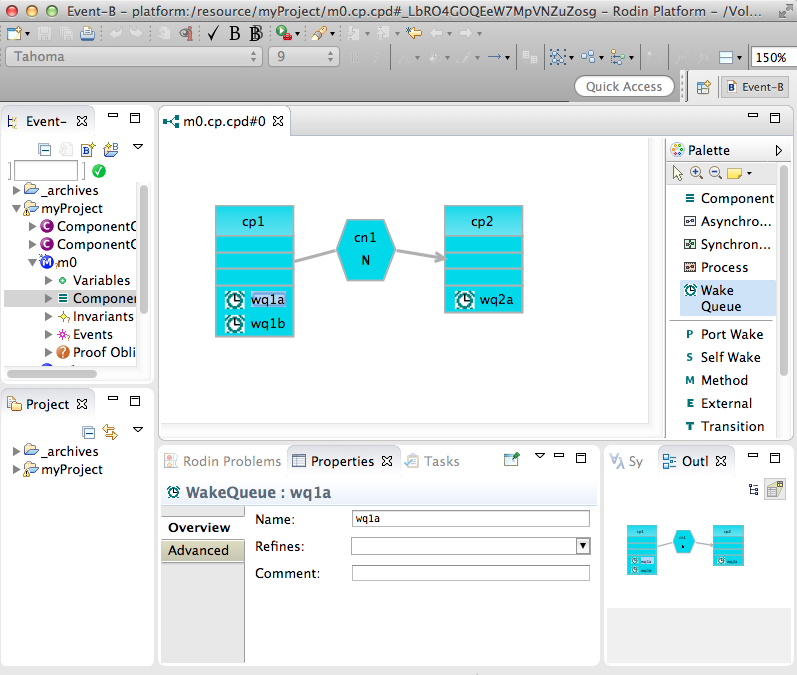
\includegraphics[width=1024]{figures/image56.png}
  \else
  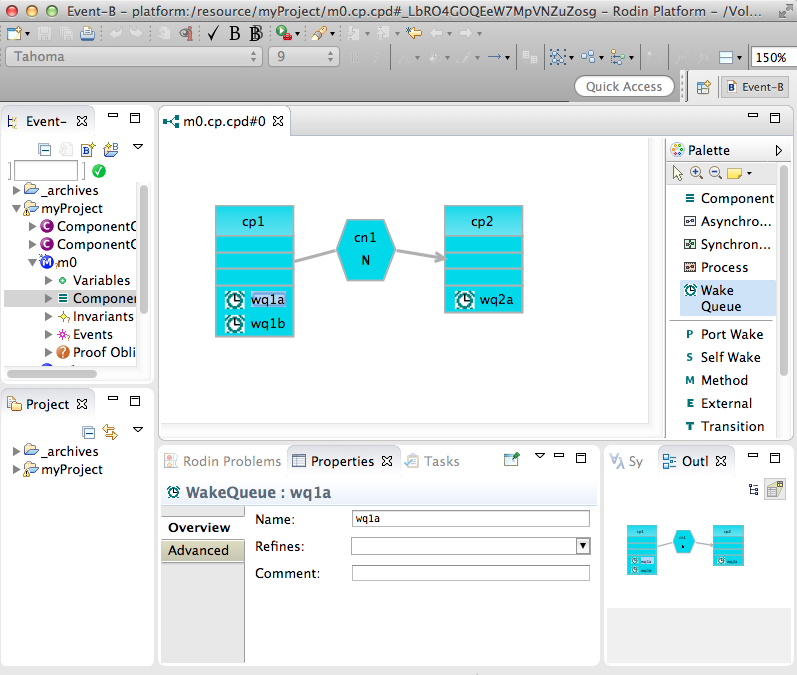
\includegraphics[width=1\textwidth]{figures/image56.png}
  \fi
  \caption{Wake Queues are added to a component using the palette}
  \label{fig:Wake QueuesAreAddedToAComponentUsingThePalette}
\end{figure}  
\begin{figure}[!htbp]
  \centering
  \ifplastex
  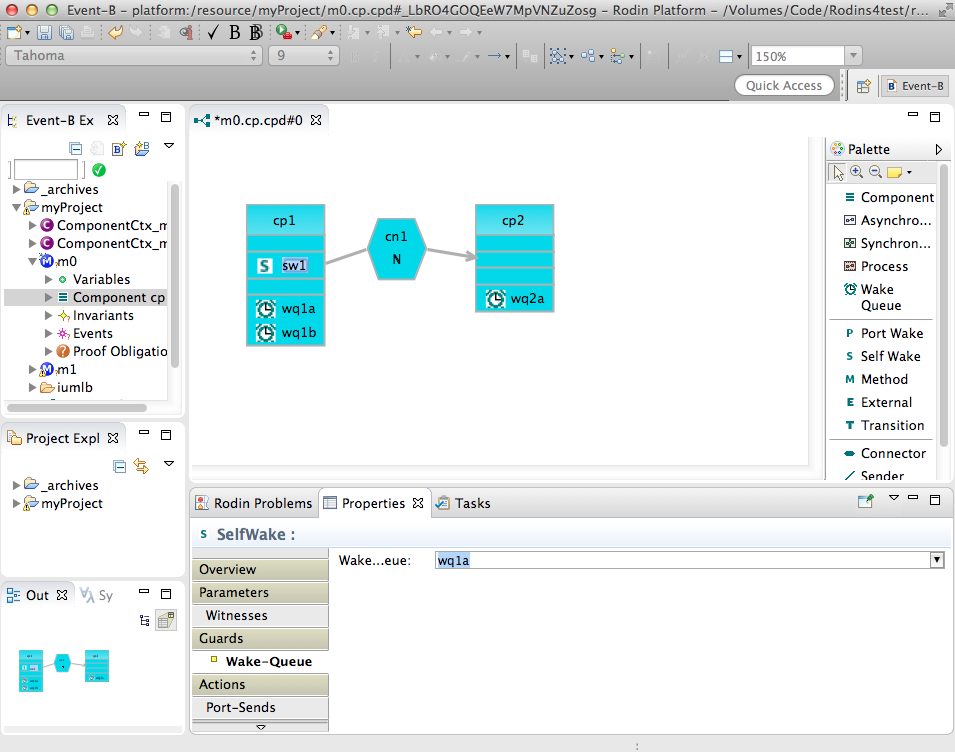
\includegraphics[width=1024]{figures/image57.png}
  \else
  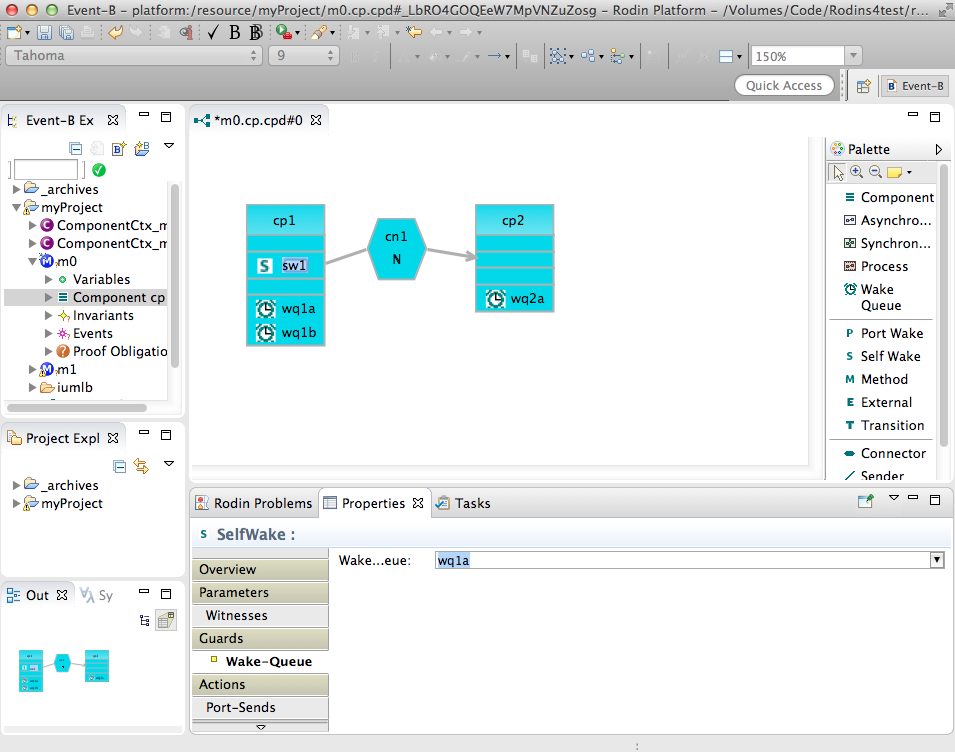
\includegraphics[width=1\textwidth]{figures/image57.png}
  \fi
  \caption{SelfWake operations must specify which of the component's wake queues they wake on}
  \label{fig:SelfWakeOperationsMustSpecifyWhichOfTheComponentsWakeQueuesTheyWakeOn}
\end{figure}  
\begin{figure}[!htbp]
  \centering
  \ifplastex
  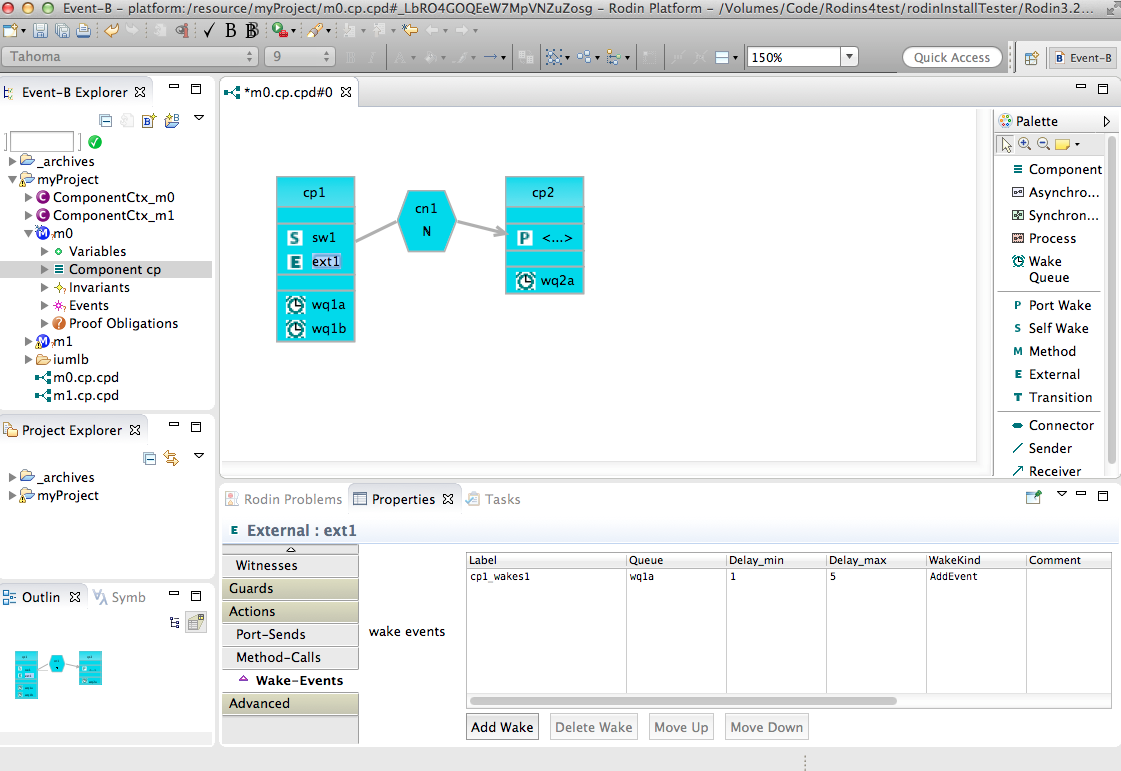
\includegraphics[width=1024]{figures/image58.png}
  \else
  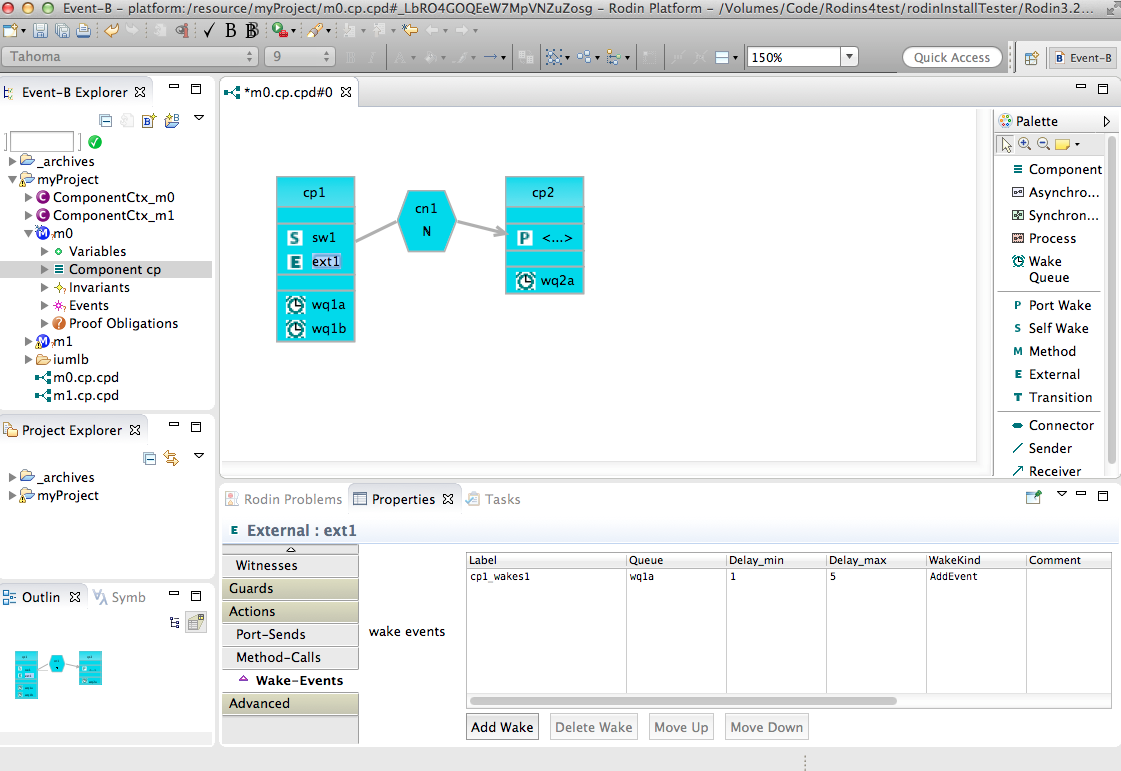
\includegraphics[width=1\textwidth]{figures/image58.png}
  \fi
  \caption{Operations that set wake events must specify which wake queue the event is set in and min and max values for the period in which the event must be dealt with by a SelfWake operation}
  \label{fig:OperationsThatSetWakeEventsMustSpecifyWhichWakeQueueTheEventIsSetIn}
\end{figure}

\subsection{Non-determinism in delay of Self Wake event}
An event in a self wake queue now consists of two time values in order to specify a time interval during which the event must be dealt with by a self wake operation (Figure \ref{fig:OperationsThatSetWakeEventsMustSpecifyWhichWakeQueueTheEventIsSetIn}).

\subsection{Process State-machines}
A third kind of state-machine is now available in CODA. Process state-machines represent a sequence of actions that make up a process and hence must complete before the next clock tick. Once a process state-machine is initiated (by linking its initial transition with an operation of the component) the timer event is disabled until it completes one of its final transitions.

\subsection{Morphing State-machines from one kind to another}
A button is provided in the properties view of component state-machines to transform a state-machine to a different kind. For example, an asynchronous state machine can be changed to a synchronous state machine in a refinement. This is needed to support the final refinement steps to allow for an HDL output.

\subsection{Renaming refined components}
The name of refined Components can now be different from the component that they refine. (Note: currently appropriate invariants have to be added to reflect the refinement of associated generated data).

\subsection{Appearance preferences}
The appearance of diagram elements can be altered, either by changing the preferences settings for component diagrams or by altering a particular element's appearance in the properties view.

\subsection{Resetting between groups of Port Wakes}
Port Wakes that listen to several connectors now reset the synchronisation flag of any other Port Wakes that are listening on a proper subset of the same connectors. 

\subsection{New features of iUML-B State-machines}
The new release of iUML-B Statemachines is adopted in CODA. This includes:\begin{itemize}
\item Junctions: allowing more flexibility in specifying or'd source states,\item Forks and Joins: allowing clearer specification of entry/exit from parallel nested state-machines, \item Any: providing a way to specify un-guarded transitions at the top level, 
\end{itemize}
\subsection{Limitations} Below are the current limitations
\begin{enumerate}
\item Refinement and subsequent refactoring needs more work (to be done in next phase). E.g. 
  \begin{itemize}
  \item Currently if any refinement needs to be made, `extends' must be manually switched off in the affected events before re-generation.	\item Invariants should be generated to reflect the refinements between components.	\item Invariants should be generated to reflect the data refinement of self-wake queues including the tightening of delay ranges.
  \end{itemize}\item In some cases invariants are repeated unnecessarily.\item Some refactoring of the code could be performed. E.g. to use the generic animation toolbar
\end{enumerate}

%%% Local Variables:
%%% mode: latex
%%% TeX-master: "component_diagrams-user_manual"
%%% End:
